\section{Objectives}
Follow Lab 9 (PDF pages 35--38): size a reference inverter, then compare two-input NAND/NOR input order, dimensions, transfer curves, noise margins, speed and power.

\section{Specification mapping}
\begin{longtable}{p{0.31\linewidth}p{0.29\linewidth}p{0.31\linewidth}}
\toprule
Handout requirement (PDF page) & Implementation & Verification and scope \\\midrule
Step 1: balance inverter (35,38) & 01\_inverter\_sizing & Ratios 3--7; select 6 \\
Steps 2/3: NAND/NOR sizing and DC (36--38) & 02\_nand, 03\_nor, 04\_sizing\_refinement & A, B, A=B; complete NM \\
Questions 1/2: late input and parasitics (38) & One input switches after the other settles & Both input positions measured \\
Question 3: factors 1.5/2/2.5/3 (38) & Four cases in 02/03 & Compare output rise/fall \\
Question 4: speed, power and area (38) & Average supply power and total widths & Equal loads; area is only a proxy \\
\bottomrule
\end{longtable}


\section{Circuit and design derivation}
Length is fixed at $0.25\,\mu$m and reference $W_n=0.6\,\mu$m. Sweep $W_p/W_n=3,4,5,6,7$ and choose 6 as the gate reference. NAND has series NMOS and parallel PMOS; NOR reverses these networks. A is nearest the output in the NAND stack and nearest the supply in the NOR stack. Each gate retains simultaneous A=B switching and the two individually sensitized inputs. The inactive input is held at 1 for NAND and 0 for NOR.

Initially, series widths are multiplied by K=1.5/2/2.5/3 to test $R\propto L/W$. Input-specific refinement then compensates for parasitic effects. The selected third refinement uses NAND PMOS A/B widths 4.14/5.04 and NMOS widths 1.5 each; NOR PMOS widths are 21.6 each and NMOS A/B widths 2.7/1.02, in $\mu$m. The source Lab9 first file incorrectly referenced an external PWM circuit; a self-contained inverter calibration replaces it. All gates include their own circuitry and measurements.

\section{Simulation setup}
This teaching rewrite uses a separately supplied model at 1.0 V and $25\,^{\circ}\mathrm C$. The specified topology, loads and comparative dimensions are retained. The handout's 2.5 V process results are not acceptance values for this model. The chosen 1 V is a simulation condition, not a verified device rating. MOS bulk terminals are explicitly connected to the corresponding supply rails.

HSPICE S-2021.09 uses RUNLVL=6, retaining waveforms, printed data and native measurements. Figures are redrawn from actual data; CSV files are in each Lab's results directory. Successful solution does not establish process reliability. Warnings from encrypted model blocks remain suppressed; the existing diagnostic did not expose actionable further details, so the warnings are not declared harmless and complete model-limit compliance is not claimed.

Every output has 20 fF. Input edges are 0.1 ns, period 5 ns; simulate 15 ns with 1 ps printing. DC is 0--1 V in 0.5 mV steps. Supply power is averaged over full cycles from 5--15 ns and excludes ideal input-source energy. NM uses the Lab8 boundary-output definition. The handout specifies approximate equality without a tolerance; 10\% is an added engineering comparison target, not a claimed original acceptance threshold.

\section{Results and specification checks}
All four decks and 16 cases completed without failed measurements.
\begin{center}\small
\begin{tabular}{llll}
\toprule
$W_p/W_n$ & $V_M$ (V) & $t_r$ (ps) & $t_f$ (ps) \\
\midrule
3 & 0.4825 & 222.64 & 110.85 \\
4 & 0.4956 & 173.83 & 113.49 \\
5 & 0.5058 & 144.13 & 115.26 \\
6 & 0.5142 & 124.85 & 117.32 \\
7 & 0.5212 & 110.93 & 119.71 \\
\bottomrule
\end{tabular}
\end{center}
\begin{center}\small
\begin{tabular}{lllll}
\toprule
Gate & Input & $V_M$ (V) & $NM_L$ (V) & $NM_H$ (V) \\
\midrule
NAND & both & 0.5464 & 0.4615 & 0.3621 \\
NAND & a & 0.4923 & 0.3924 & 0.4226 \\
NAND & b & 0.4827 & 0.3808 & 0.4331 \\
NOR & both & 0.4792 & 0.3849 & 0.4430 \\
NOR & a & 0.5455 & 0.4539 & 0.3585 \\
NOR & b & 0.5352 & 0.4442 & 0.3712 \\
\bottomrule
\end{tabular}
\end{center}

\begin{figure}[htbp]
\centering
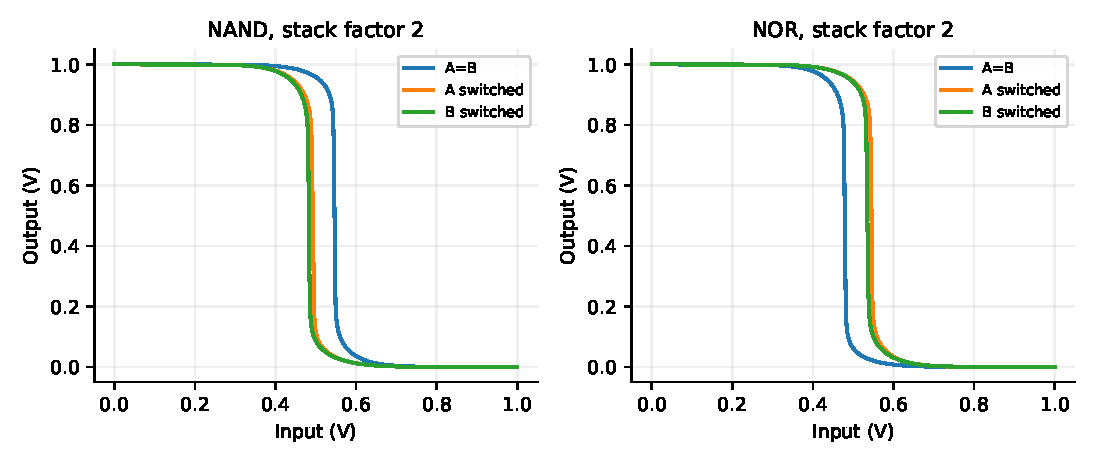
\includegraphics[width=\linewidth]{figures/gate_transfer.pdf}
\caption{Three input conditions with stack factor 2; redrawn from this run's HSPICE data.}
\end{figure}
\begin{center}\small
\begin{tabular}{lllll}
\toprule
Selected design & $t_r$ (ps) & $t_f$ (ps) & $t_{pHL}$ (ps) & $t_{pLH}$ (ps) \\
\midrule
INV & 123.30 & 116.03 & 109.74 & 96.30 \\
NAND A & 130.26 & 111.14 & 99.02 & 102.50 \\
NAND B & 124.24 & 111.18 & 107.10 & 104.32 \\
NOR A & 134.89 & 122.00 & 135.99 & 121.49 \\
NOR B & 128.66 & 116.35 & 150.46 & 79.97 \\
\bottomrule
\end{tabular}
\end{center}

\begin{figure}[htbp]
\centering
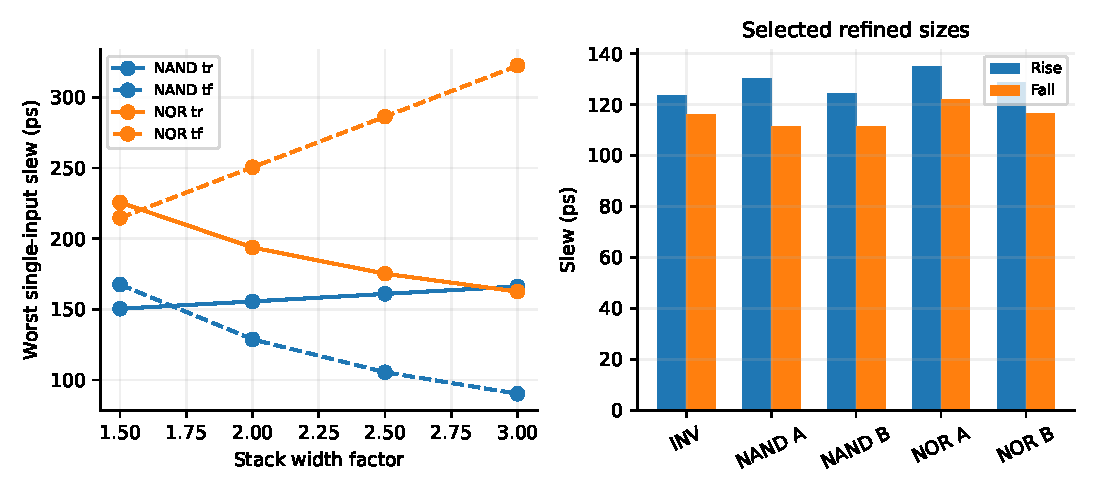
\includegraphics[width=\linewidth]{figures/gate_sizing.pdf}
\caption{Stack-factor sweep and final size refinement; redrawn from this run's HSPICE data.}
\end{figure}
Mean supply power and total widths at initial K=2:
\begin{center}\small
\begin{tabular}{lllll}
\toprule
Gate & $P_{A=B}$ ($\mu$W) & $P_A$ ($\mu$W) & $P_B$ ($\mu$W) & $\sum W$ ($\mu$m) \\
\midrule
NAND & 7.145 & 6.480 & 7.299 & 9.6 \\
NOR & 9.134 & 12.916 & 7.232 & 15.6 \\
\bottomrule
\end{tabular}
\end{center}


\section{Discussion}
The ratio-6 inverter has a threshold near 0.514 V and rise/fall times of about 124.85/117.32 ps: close, not perfectly symmetric. In the selected refinement, the maximum single-input slew deviation from the same-deck inverter is about 9.4\%. Simultaneous activation of parallel devices is faster, so equality across every input mode is not expected.

The latest signal should drive the series device nearest the output: A for NAND, B for NOR. The other input is held settled in this test. Internal-node charging and body effect make simple stack-count width multiplication inexact; widening also increases junction, overlap and input capacitance. At initial K=2, total widths are 9.6 for NAND and 15.6 $\mu$m for NOR. This is an active-width proxy at equal L, excluding layout, contacts and routing. CSV files retain average supply power for every input mode. NOR is generally slower and more energy-consuming in this equal-load comparison, but no universal cross-process ranking is claimed. Matching slew by greatly enlarging NOR trades area and input loading for speed.

\section{Conclusion}
All three steps and four questions have corresponding tests. The specified multipliers are retained before further refinement. Approximate 10\% matching is a result against this run's added engineering target; original-process values and unknown reliability constraints are not declared satisfied.
